\documentclass[]{article}
\usepackage[left=1in,top=1in,right=1in,bottom=1in]{geometry}


%%%% more monte %%%%
% thispagestyle{empty}
% https://stackoverflow.com/questions/2166557/how-to-hide-the-page-number-in-latex-on-first-page-of-a-chapter
\usepackage{color}
% \usepackage[table]{xcolor} % are they using color?

% \definecolor{WSU.crimson}{HTML}{981e32}
% \definecolor{WSU.gray}{HTML}{5e6a71}

% \definecolor{shadecolor}{RGB}{248,248,248}
\definecolor{WSU.crimson}{RGB}{152,30,50} % use http://colors.mshaffer.com to convert from 981e32
\definecolor{WSU.gray}{RGB}{94,106,113}

%%%%%%%%%%%%%%%%%%%%%%%%%%%%

\newcommand*{\authorfont}{\fontfamily{phv}\selectfont}
\usepackage{lmodern}


  \usepackage[T1]{fontenc}
  \usepackage[utf8]{inputenc}




\usepackage{abstract}
\renewcommand{\abstractname}{}    % clear the title
\renewcommand{\absnamepos}{empty} % originally center

\renewenvironment{abstract}
 {{%
    \setlength{\leftmargin}{0mm}
    \setlength{\rightmargin}{\leftmargin}%
  }%
  \relax}
 {\endlist}

\makeatletter
\def\@maketitle{%
  \pagestyle{empty}
  \newpage
%  \null
%  \vskip 2em%
%  \begin{center}%
  \let \footnote \thanks
    {\fontsize{18}{20}\selectfont\raggedright  \setlength{\parindent}{0pt} \@title \par}%
}
%\fi
\makeatother






\usepackage{color}
\usepackage{fancyvrb}
\newcommand{\VerbBar}{|}
\newcommand{\VERB}{\Verb[commandchars=\\\{\}]}
\DefineVerbatimEnvironment{Highlighting}{Verbatim}{commandchars=\\\{\}}
% Add ',fontsize=\small' for more characters per line
\usepackage{framed}
\definecolor{shadecolor}{RGB}{248,248,248}
\newenvironment{Shaded}{\begin{snugshade}}{\end{snugshade}}
\newcommand{\AlertTok}[1]{\textcolor[rgb]{0.94,0.16,0.16}{#1}}
\newcommand{\AnnotationTok}[1]{\textcolor[rgb]{0.56,0.35,0.01}{\textbf{\textit{#1}}}}
\newcommand{\AttributeTok}[1]{\textcolor[rgb]{0.77,0.63,0.00}{#1}}
\newcommand{\BaseNTok}[1]{\textcolor[rgb]{0.00,0.00,0.81}{#1}}
\newcommand{\BuiltInTok}[1]{#1}
\newcommand{\CharTok}[1]{\textcolor[rgb]{0.31,0.60,0.02}{#1}}
\newcommand{\CommentTok}[1]{\textcolor[rgb]{0.56,0.35,0.01}{\textit{#1}}}
\newcommand{\CommentVarTok}[1]{\textcolor[rgb]{0.56,0.35,0.01}{\textbf{\textit{#1}}}}
\newcommand{\ConstantTok}[1]{\textcolor[rgb]{0.00,0.00,0.00}{#1}}
\newcommand{\ControlFlowTok}[1]{\textcolor[rgb]{0.13,0.29,0.53}{\textbf{#1}}}
\newcommand{\DataTypeTok}[1]{\textcolor[rgb]{0.13,0.29,0.53}{#1}}
\newcommand{\DecValTok}[1]{\textcolor[rgb]{0.00,0.00,0.81}{#1}}
\newcommand{\DocumentationTok}[1]{\textcolor[rgb]{0.56,0.35,0.01}{\textbf{\textit{#1}}}}
\newcommand{\ErrorTok}[1]{\textcolor[rgb]{0.64,0.00,0.00}{\textbf{#1}}}
\newcommand{\ExtensionTok}[1]{#1}
\newcommand{\FloatTok}[1]{\textcolor[rgb]{0.00,0.00,0.81}{#1}}
\newcommand{\FunctionTok}[1]{\textcolor[rgb]{0.00,0.00,0.00}{#1}}
\newcommand{\ImportTok}[1]{#1}
\newcommand{\InformationTok}[1]{\textcolor[rgb]{0.56,0.35,0.01}{\textbf{\textit{#1}}}}
\newcommand{\KeywordTok}[1]{\textcolor[rgb]{0.13,0.29,0.53}{\textbf{#1}}}
\newcommand{\NormalTok}[1]{#1}
\newcommand{\OperatorTok}[1]{\textcolor[rgb]{0.81,0.36,0.00}{\textbf{#1}}}
\newcommand{\OtherTok}[1]{\textcolor[rgb]{0.56,0.35,0.01}{#1}}
\newcommand{\PreprocessorTok}[1]{\textcolor[rgb]{0.56,0.35,0.01}{\textit{#1}}}
\newcommand{\RegionMarkerTok}[1]{#1}
\newcommand{\SpecialCharTok}[1]{\textcolor[rgb]{0.00,0.00,0.00}{#1}}
\newcommand{\SpecialStringTok}[1]{\textcolor[rgb]{0.31,0.60,0.02}{#1}}
\newcommand{\StringTok}[1]{\textcolor[rgb]{0.31,0.60,0.02}{#1}}
\newcommand{\VariableTok}[1]{\textcolor[rgb]{0.00,0.00,0.00}{#1}}
\newcommand{\VerbatimStringTok}[1]{\textcolor[rgb]{0.31,0.60,0.02}{#1}}
\newcommand{\WarningTok}[1]{\textcolor[rgb]{0.56,0.35,0.01}{\textbf{\textit{#1}}}}



\title{\textbf{\textcolor{WSU.crimson}{The Influence of Biological Sex
on Human Body Part Ratios}} \newline \textbf{\textcolor{WSU.gray}{How
these Ratios Compare Between the Sexes}}  }
 

%  

% \author{ \Large true \hfill \normalsize \emph{} }
\author{\Large Kevin A. Black -
\href{mailto:kevin.black@wsu.edu}{\nolinkurl{kevin.black@wsu.edu}}\vspace{0.05in} \newline\normalsize\emph{Washington
State University Vancouver}  }


\date{November 05, 2020}
\setcounter{secnumdepth}{3}

\usepackage{titlesec}
% See the link above: KOMA classes are not compatible with titlesec any more. Sorry.
% https://github.com/jbezos/titlesec/issues/11
\titleformat*{\section}{\bfseries}
\titleformat*{\subsection}{\bfseries\itshape}
\titleformat*{\subsubsection}{\itshape}
\titleformat*{\paragraph}{\itshape}
\titleformat*{\subparagraph}{\itshape}

% https://code.usgs.gov/usgs/norock/irvine_k/ip-092225/


%\titleformat*{\section}{\normalsize\bfseries}
%\titleformat*{\subsection}{\normalsize\itshape}
%\titleformat*{\subsubsection}{\normalsize\itshape}
%\titleformat*{\paragraph}{\normalsize\itshape}
%\titleformat*{\subparagraph}{\normalsize\itshape}

% https://tex.stackexchange.com/questions/233866/one-column-multicol-environment#233904
\usepackage{environ}
\NewEnviron{auxmulticols}[1]{%
  \ifnum#1<2\relax% Fewer than 2 columns
    %\vspace{-\baselineskip}% Possible vertical correction
    \BODY
  \else% More than 1 column
    \begin{multicols}{#1}
      \BODY
    \end{multicols}%
  \fi
}





\usepackage{natbib}
\setcitestyle{aysep={}} %% no year, comma just year
% \usepackage[numbers]{natbib}
\bibliographystyle{./../biblio/ormsv080.bst}



\usepackage[strings]{underscore} % protect underscores in most circumstances




\newtheorem{hypothesis}{Hypothesis}
\usepackage{setspace}


%%%%%%%%%%%%%%%%%%%%%%%%%%%%%%%%%%%%%%%%%%%%%%%%%%%%%
%%% MONTE ADDS %%%

\usepackage{fancyhdr} % fancy header 
\usepackage{lastpage} % last page 

\usepackage{multicol}


\usepackage{etoolbox}
\AtBeginEnvironment{quote}{\singlespacing\small}
% https://tex.stackexchange.com/questions/325695/how-to-style-blockquote


\usepackage{soul}			%% allows strike-through
\usepackage{url}			%% fixes underscores in urls
\usepackage{csquotes}		%% allows \textquote in references
\usepackage{rotating}		%% allows table and box rotation
\usepackage{caption}		%% customize caption information
\usepackage{booktabs}		%% enhance table/tabular environment
\usepackage{tabularx}		%% width attributes updates tabular
\usepackage{enumerate}		%% special item environment
\usepackage{enumitem}		%% special item environment

\usepackage{lineno}		%% allows linenumbers for editing using \linenumbers
\usepackage{hanging}


\usepackage{mathtools}  	%% also loads amsmath
\usepackage{bm}		%% bold-math
\usepackage{scalerel}	%% scale one element (make one beta bigger font)

\newcommand{\gFrac}[2]{ \genfrac{}{}{0pt}{1}{{#1}}{#2} }

\newcommand{\betaSH}[3]{  \gFrac{\text{\tiny #1}}{{\text{\tiny #2}}}\hat{\beta}_{\text{#3}}   }
\newcommand{\betaSB}[3]{              ^{\text{#1}} _{\text{#2}} \bm{\beta} _{\text{#3}}                   }  %% bold
\newcommand{\bigEQ}{  \scaleobj{1.5}{{\ }= } }
\newcommand{\bigP}[1]{  \scaleobj{1.5}{#1 } }





\usepackage{endnotes}  % he already does this ...
\renewcommand{\enotesize}{\normalsize}
% https://tex.stackexchange.com/questions/99984/endnotes-do-not-be-superscript-and-add-a-space
\renewcommand\makeenmark{\textsuperscript{[\theenmark]}} % in brackets %
% https://tex.stackexchange.com/questions/31574/how-to-control-the-indent-in-endnotes
\patchcmd{\enoteformat}{1.8em}{0pt}{}{}

\patchcmd{\theendnotes}
  {\makeatletter}
  {\makeatletter\renewcommand\makeenmark{\textbf{[\theenmark]} }}
  {}{}



% https://tex.stackexchange.com/questions/141906/configuring-footnote-position-and-spacing

\addtolength{\footnotesep}{5mm} % change to 1mm

\renewcommand{\thefootnote}{\textbf{\arabic{footnote}}}
\let\footnote=\endnote
%\renewcommand*{\theendnote}{\alph{endnote}}
%\renewcommand{\theendnote}{\textbf{\arabic{endnote}}}


\renewcommand*{\notesname}{ENDNOTES}

\makeatletter
\def\enoteheading{\section*{\notesname
  \@mkboth{\MakeUppercase{\notesname}}{\MakeUppercase{\notesname}}}%
  \mbox{}\par\vskip-2.3\baselineskip\noindent\rule{.5\textwidth}{0.4pt}\par\vskip\baselineskip}
\makeatother


\renewcommand*{\contentsname}{TABLE OF CONTENTS}

\renewcommand*{\refname}{REFERENCES}


%\usepackage{subfigure}
\usepackage{subcaption}

\captionsetup{labelfont=bf}  % Make Table / Figure bold

%%% you could add elements here ... monte says .... %%%
%\usepackage{mypackageForCapitalH}


%%%%%%%%%%%%%%%%%%%%%%%%%%%%%%%%%%%%%%%%%%%%%%%%%%%%%

% set default figure placement to htbp
\makeatletter
\def\fps@figure{htbp}
\makeatother

\usepackage{hyperref}

% move the hyperref stuff down here, after header-includes, to allow for - \usepackage{hyperref}

\makeatletter
\@ifpackageloaded{hyperref}{}{%
\ifxetex
  \PassOptionsToPackage{hyphens}{url}\usepackage[setpagesize=false, % page size defined by xetex
              unicode=false, % unicode breaks when used with xetex
              xetex]{hyperref}
\else
  \PassOptionsToPackage{hyphens}{url}\usepackage[draft,unicode=true]{hyperref}
\fi
}

\@ifpackageloaded{color}{
    \PassOptionsToPackage{usenames,dvipsnames}{color}
}{%
    \usepackage[usenames,dvipsnames]{color}
}
\makeatother
\hypersetup{breaklinks=true,
            bookmarks=true,
            pdfauthor={Kevin A. Black -
\href{mailto:kevin.black@wsu.edu}{\nolinkurl{kevin.black@wsu.edu}} (Washington
State University Vancouver)},
             pdfkeywords = {Shapiro-Wilk test, Pearson Product-Moment
Correlation, null hypothesis, alternative hypothesis, two-sample t-test,
data provenance.},  
            pdftitle={The Influence of Biological Sex on Human Body Part
Ratios: How these Ratios Compare Between the Sexes},
            colorlinks=true,
            citecolor=blue,
            urlcolor=blue,
            linkcolor=magenta,
            pdfborder={0 0 0}}
\urlstyle{same}  % don't use monospace font for urls

% Add an option for endnotes. -----

%
% add tightlist ----------
\providecommand{\tightlist}{%
\setlength{\itemsep}{0pt}\setlength{\parskip}{0pt}}

% add some other packages ----------

% \usepackage{multicol}
% This should regulate where figures float
% See: https://tex.stackexchange.com/questions/2275/keeping-tables-figures-close-to-where-they-are-mentioned
\usepackage[section]{placeins}



\pagestyle{fancy}   
\lhead{\textcolor{WSU.crimson}{\textbf{ The Influence of Biological Sex
on Human Body Part Ratios }}}
\chead{}
\rhead{\textcolor{WSU.gray}{\textbf{  Page\ \thepage\ of\ \protect\pageref{LastPage} }}}
\lfoot{}
\cfoot{}
\rfoot{}


\begin{document}
	
% \pagenumbering{arabic}% resets `page` counter to 1 
%    

% \maketitle

{% \usefont{T1}{pnc}{m}{n}
\setlength{\parindent}{0pt}
\thispagestyle{plain}
{\fontsize{18}{20}\selectfont\raggedright 
\maketitle  % title \par  

}

{
   \vskip 13.5pt\relax \normalsize\fontsize{11}{12} 
   
\textbf{\authorfont Kevin A. Black -
\href{mailto:kevin.black@wsu.edu}{\nolinkurl{kevin.black@wsu.edu}}} \hskip 15pt \emph{\small Washington
State University Vancouver}   

}

}








\begin{abstract}

    \hbox{\vrule height .2pt width 39.14pc}

    \vskip 8.5pt % \small 

\noindent Throughout history, there have been evident traits of
uniqueness among the multicellular organisms that roam the Earth. A
common theme among these creatures relates to the differences in
biological sexes, especially when it comes to size or behavior. In an
endeavor to establish some distinct patterns between the biological
sexes of humans, male and female, students of the STAT 419 course
(Introduction to Multivariate Statistics) at Washington State University
conducted a large-scale survey amongst each other and their peers. This
brief survey was composed of body part measurements and other metrics
like gender, ethniticty, eye color, age, and so on. The students
recorded the data in a consistent format, which was then compiled by the
instructor of the class, Monte Shaffer. After the compilation of data,
students were free to formulate their own questions and look for
recognizable patterns amongst the values. These students also practiced
data provenance whilst conducting their research to make sure the body
measurement data wasn't misused in the process.

\vspace{0.25cm}

For this research paper in particular, I address the topic of how
biological sex influences the ratios of particular body parts.
Specifically, this paper looks at the influence that being male or
female has on two body measurement ratios: (1) the ratio of height and
arm span and (2) the ratio of height and head height. The steps taken in
this research involved performing a Pearson correlation test on the
ratio of height and arm span, while a two-sample t-test was performed on
the ratio of height and head height. The results of these tests found
that while there was a noticeable variation in the measurements of male
and female body parts, the previously mentioned ratios were very
similar, which fall in line with our current body proportion knowledge
for biological males and females.


\vskip 8.5pt \noindent \textbf{\underline{Keywords}:} Shapiro-Wilk test,
Pearson Product-Moment Correlation, null hypothesis, alternative
hypothesis, two-sample t-test, data provenance. \par

    




    
    \hbox{\vrule height .2pt width 39.14pc}
    \vskip 5pt 
    \hfill \textbf{\textcolor{WSU.gray}{ November 05, 2020 } }
    \vskip 5pt 
    
\end{abstract}


\vskip -8.5pt



 % removetitleabstract

\noindent  

\section{Introduction}
\label{sec:intro}

As a customary portion of the STAT 419 course at Washington State
University, the course students involved were required to take part in a
data collection/manipulation project involving the measurements of
various body parts. Following the data collection, professor Monte
Shaffer compiled all student contributions into a single, pipe-delimited
text file whose explicit content is to remain confidential and only used
for the sake of addressing the research questions presented in this
paper.

\vspace{0.25cm}

After receiving the data set (\(n=428\)) and cleaning up particular
observations using a range of methodologies based on what I had in mind
for how this data will be used, I determined that I would focus on what
kind of influence biological sex has on certain human body part ratios.
To supplement my inquiry of this data, I centered my research questions
around particular parts of the human body, which would be \(height\),
\(arm.span\), and \(head.height\) of the data set. These variables
correspond to the standing height of the individual with no shoes on,
the length from one middle finger to the other with fully extended arms,
and the height from the top of the head to below the chin, respectively.
Research questions pertaining to this study begins in section
\ref{sec:rq} and supportive R code can be found in section
\ref{sec:r-setup}.

\section{Data Description}
\label{sec:data}

As mentioned in the introduction, the data set utilized throughout this
research paper was supplied through the combined efforts of professor
Monte Shaffer and the students of the STAT 419 class at Washington State
University. Each student was tasked with recording observations composed
of 37 attributes from 10 different people, ideally with an even mix of
males and females. For each observation (denoted as an individual
person), there are measurements of body parts, data collector/respondent
identifiers ran through a MD5 hash function, and general information
about each respondent. Body part measurements were recorded with body
measuring tape and in particular units up to the surveyor's personal
choice (either inches or centimeters). For the sake of consistency
throughout this research paper, all centimeter values were converted to
inches and measurement values will be treated as inches from here on.

\vspace{0.25cm}

These observations were recorded in early September 2020 and compiled by
the instructor for our use in late October 2020. Given that these
observations were recorded amid the COVID-19 pandemic, each student was
required to make a simple, yet descriptive handout that would detail how
one would go about recording their own body measurements and the
necessary values to take note of. This would be an ideal situation of
how observations were recorded and sent electronically by each
respondent, but observations could also be taken in person given that
the surveyor and respondent were comfortable being in close proximity of
each other. An example of a two-page handout created by Kevin Black, as
well as further information regarding the attributes of this data set,
can be found in Appendix \ref{sec:appendix-data-handout} and Appendix
\ref{sec:appendix-dataset-ex}, respectively.

\vspace{0.25cm}

On the surface, the purpose for writing this research paper and
collecting the necessary data can simply be attributed to project
requirements for a university course. However, the deeper reasoning
behind why this research paper was created in the first place was to
give students a more thorough understanding of the data analytics
process. More specifically, how to not just work with the data, but how
to understand the data and derive effective questions, what kind of data
to wrangle for particular research, how to properly clean data, how to
test for patterns and conclusions in a statistical, analytic
environment, and how to exercise data provenance practices. This process
will be very similar between all data focused projects in a data
analyst's career, so this was a good starting point for garnering
crucial experience.

\section{How does being male or female influence the ratios between certain body parts?}
\label{sec:rq}

Generally, making particular deductions about body measurements among
males and females is more than likely due to the distinct physical
patterns one can find when comparing the biological sexes. Those born
biologically as males or females have about as many differing features
to one another than their similar features, both internally and
externally. Internally speaking, men typically have deeper voices, a
faster metabolism, and can easily build muscle mass, whereas women
possess a much more sophisticated reproductive system, possess the
ability to breastfeed, and live longer on average
\citep{Wolchover:2011}. Now what about externally? How does being male
or female influence the ratios between certain body parts? The latter
primary question will be elaborated through the following sub-questions,
focusing on particular ratios that are likely to yield some insight on
the different external measurements between males and females.

\subsection{How does 'height' compare to 'arm span' between males and females?}
\label{sec:rq2}

The body part ratio between \(height\) and \(arm.span\) is a well-known
one where ``for most people, their arm span is about equal to their
height. Mathematicians say the arm span to height ratio is one to one''
\citep{Brabandere:2017}. To set up this sub-question, let's first
declare some null and alternative hypotheses for males and females. For
males, \(H_0:\rho_m=0\) and \(H_1:\rho_m\neq0\). For females,
\(H_0:\rho_f=0\) and \(H_1:\rho_f\neq0\). We must also check both
vectors for normality prior to correlation testing by performing a
Shapiro-Wilk test with the \texttt{shapiro.test()} function. Running
this function gives results for males \(height\) (\(W=0.73255\),
\(p=2.303\times10^{-11}\)) and \(arm.span\) (\(W=0.80943\),
\(p=2.664\times10^{-9}\)), as well as for females \(height\)
(\(W=0.78534\), \(p=6.762\times10^{-11}\)) and \(arm.span\)
(\(W=0.82018\), \(p=8.305\times10^{-10}\)). All of these test statistics
show that we can move forward with the \texttt{cor.test()} function as
each of these tested populations may come from normal distributions. The
correlation test will be conducted using the method of Pearson
Product-Moment Correlation.

\vspace{0.25cm}

Given the results of \texttt{cor.test()}, when it comes to males we
reject our null hypothesis \(H_0:\rho_m=0\) and accept our alternative
hypothesis \(H_1:\rho_m\neq0\) as there is some clear indication of
strong, positive correlation among the male body parts
(\(t_{86}=33.105\), \(p<2.2\times10^{-16}\)). The same conclusion can be
made with females, where we reject our null hypothesis \(H_0:\rho_f=0\)
and accept our alternative hypothesis \(H_1:\rho_f\neq0\)
(\(t_{100}=40.488\), \(p<2.2\times10^{-16}\)). Based solely on figure
\ref{fig:sq1} below that was generated from the R code in section
\ref{sec:first-subq}, we can see that there are strong positive
correlations for both males and females with regard to their respective
\(height\) and \(arm.span\) values. Additionally, a table displaying the
mean, standard deviation, and correlation values for the male and female
body parts used in this study can be found in section
\ref{sec:correlation-tables}.

\begin{figure}[!ht]
    \begin{center}
        \scalebox{1.00}{    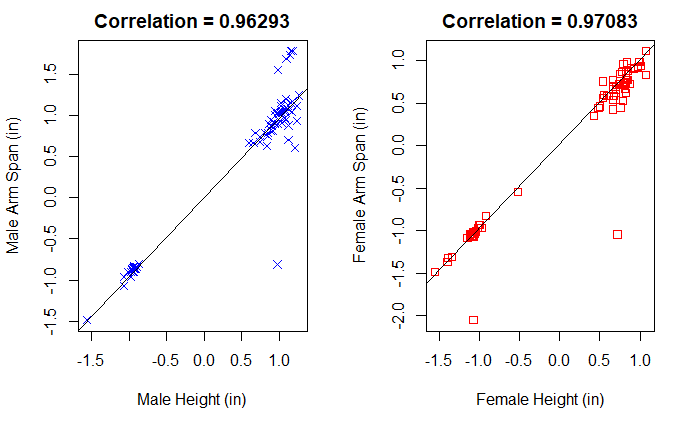
\includegraphics[trim = 0 0 0 0,clip,width=0.85\textwidth]{figures/sq1.png} }
        \caption{Plots/correlation values for males and females regarding $height$ and $arm.span$.}
        \label{fig:sq1}
    \end{center}
\end{figure}

\subsection{How many average 'head height' lengths are males and females relative to their respective, average 'height'?}
\label{sec:rq4}

To form the foundation for how we'll go about answering this second
sub-question, let's consider the population means for \(head.height\)
and \(height\) for males and females. To test the two population means
for equality between males and females, we will utilize a two-sample
t-test. The null hypotheses and alternative hypotheses can be set up as
follows:

\begin{itemize}
\item
  Regarding \(head.height\), to determine if the population means for
  males and females are equal, let the null hypothesis be
  \(H_0: \mu_{m.head}=\mu_{f.head}\) and the alternative hypothesis be
  \(H_1: \mu_{m.head} \neq \mu_{f.head}\).
\item
  Regarding \(height\), to determine if the population means for males
  and females are equal, let the null hypothesis be
  \(H_0: \mu_{m.height}=\mu_{f.height}\) and the alternative hypothesis
  be \(H_1: \mu_{m.height} \neq \mu_{f.height}\).
\end{itemize}

Based on the two-sample t-test results generated by the code in section
\ref{sec:second-subq}, regarding the comparison of mean \(head.height\)
between males and females, we can reject our null hypothesis
\(H_0: \mu_{m.head}=\mu_{f.head}\) and accept our null hypothesis
\(H_1: \mu_{m.head} \neq \mu_{f.head}\) as there is evidence of at least
one statistical difference in the mean head heights between the sexes
(\(t_{182.64}=3.8231\), \(p=1.807\times10^{-4}\)). And as for
\(height\), we can make a similar conclusion where we reject our null
hypothesis \(H_0: \mu_{m.height}=\mu_{f.height}\) and accept our null
hypothesis \(H_1: \mu_{m.height} \neq \mu_{f.height}\) as there is also
evidence of at least one statistical difference in the mean heights
between the sexes (\(t_{184.65}=3.9891\), \(p=9.552\times10^{-5}\)).

\vspace{0.25cm}

Now that it's established that there are indeed statistical differences
between males and females when it comes to their respective mean
\(head.height\) and \(height\) values, we can calculate the explicit
values to determine how many average \(head.height\) lengths males and
females are relative to their respective, average \(height\). From the
results generated by the code in section \ref{sec:second-subq}, we can
see that the average head height for males is 18.19722 inches and for
females is 14.31103 inches, whereas the average height for males is
138.7041 inches and for females is 107.5450 inches. Using simple
division, we can describe these \(height\) values in terms of
\(head.height\) by calculating \(138.7041/18.19722\) for males and
\(107.5450/14.31103\) for females. On average, this leads to males being
7.622273 heads tall and females 7.514837 heads tall.

\newpage

\section{Key Findings}
\label{sec:findings}

For the first sub-question, the correlation between \(height\) and
\(arm.span\) measured in at 0.96293 for males and ever-so-slightly
higher at 0.97083 for females. These values mean that the heights and
arm spans for both sexes change at almost the same rate as one another,
indicating that there is little to no difference between males and
females for this common body ratio. The only distinction between the
sexes in this sample is that they operate on different value ranges,
where height and arm span are larger for males than for females. As for
the second sub-question, the surprisingly about-equal results of
7.622273 heads for males and 7.514837 heads for females lines up with
common proportion knowledge about human height in terms of head height,
where ``the average adult human is technically seven-and-one-half heads
tall\ldots{} the average adult female is smaller than the average adult
male, however you'll notice that they are both proportionately similar''
\citep{Larson:2014}.

\section{Conclusion}
\label{sec:conclusion}

It's important to reiterate that there's no doubt that males and females
can have quite stark differences when it comes to the measurements of
external features, and the research conducted above shows that while
there can be some differences, there are also some notable similarities.
For the correlation values of these particular attributes and samples,
it would appear that males and females are almost equally as likely to
have a height matching their arm span. This shows that males and females
can have a very similar body part ratio despite having varied body
measurements. The research conducted for this sub-question is simply a
supplement to information that has already been known throughout history
and simply reaffirms the existing beliefs for this specific ratio of
body parts. Lastly, for the heights of males and females measured in
terms of their respective head heights, they once again both have very
similar ratios despite them having very different average, respective
values of \(height\) and \(head.height\). The evidence provided shows
that even though males and females can have varying body measurements
between each other as a group, the influence of biological sex on human
body part ratios is seemingly non-existent in the case of these
attributes as the ratios were strikingly similar in both research
questions.

\newpage

\section{APPENDICES}
\label{sec:appendix}

\subsection{Data Provenance}
\label{sec:appendix-data-provenance}

\subsubsection{Utilization of Data Provenance}
\label{sec:appendix-provenance-explained}

While it could be seen as an application mainly used in large-scale data
analytics projects, the multitude of steps to practice data provenance
was also used to handle the vulnerable data used in this research.
Auxiliary files such as the R project files can be found on the
\href{https://github.com/KevnBlack/WSU_STATS419_FALL2020/tree/master/PROJECT-01}{project repository}
through GitHub, while the specific functions used in this report can be
found in the \texttt{functions-project-measure.R}
\href{https://bit.ly/3k1tYRj}{file} or in section
\ref{sec:functions}\footnote{The buildLatexCorrelationTable() function was a crucial function that was used to construct the table found in section \ref{sec:correlation-tables}, but it was omitted from appearing in section \ref{sec:functions} due to the length of the code involved. Instead, code for this function can be found on Monte Shaffer's Github repository through this \href{https://bit.ly/361qokY}{link}.}.
The data set itself was not saved to any location online due to privacy
concerns, but it was organized and saved onto a local hard drive for
immediate use.

\vspace{0.25cm}

The collection and general organization process for the data set is
thoroughly described in sections \ref{sec:data} and
\ref{sec:appendix-dataset-ex}. Cleaning for the actual substance of the
data set was performed through the use of the
\texttt{prepareMeasureData()} function, where the data set was
manipulated to more better fit the aims of addressing the particular
research questions for this report. Cleaning this data set involved
multiple steps, such as: omitting rows containing NA values based solely
on the body measurement columns, setting a consistent naming convention
for \(gender\) and \(units\), converting all body measurement values to
inches, and implementing the option for scaling the body measurement
data. Despite the cleaning of all columns, the only attributes that kept
the research questions in mind were retained, so the only measurement
fields utilized were \(height\), \(arm.span\), \(head.height\), and
\(gender\).

\vspace{0.25cm}

Prior to \texttt{prepareMeasureData()}, the data is imported via the
\texttt{read.file()} function where it checks to see if a cleaned
version of the data set already exists, to which that particular file
would take precedence and be
used\footnote{As mentioned in a comment in section \ref{sec:sourcing}, if you are going to change the $scale$ value from TRUE to FALSE or vice versa when invoking read.file(), be sure to remove the previous measure file from whatever you set the working directory to in the $path.to.secret$ variable. This is because no feature was implemented to remove the previous file after switching the value of $scale$ due to time constraints.}.
If no clean version currently exists, the function goes through the
cleaning process and saves the cleaned data set to the same directory as
original data set, stored in path.to.secret. For unbiased samples of the
data frame, a seed of 1 was set for reproducibility and 200 random
observations were drawn without replacement.

\vspace{0.25cm}

The documented R code can be found in section \ref{sec:r-setup}. Key
findings and visualizations of summary statistics were discussed
previously throughout sections \ref{sec:rq} through \ref{sec:findings},
as well as section \ref{sec:correlation-tables}. Based on the points
made in this section, its clear that data provenance was kept in mind
for making sure there was a traceable history in the usage of this data
set, whether to resolve potential issues or to cut down on access
times\footnote{Access times were not a huge problem for this data set as the original size of the data set was only composed of 428 observations and the research code was executed on a fairly high-end computer, however it makes for good practice when it comes time to work on larger data sets down the road.}.

\newpage

\subsubsection{Data Collection Handout}
\label{sec:appendix-data-handout}

\begin{figure}[!ht]
    \hrule
    \caption{ \textbf{Handout Page 1} }
    \begin{center}
        \scalebox{1.00}{    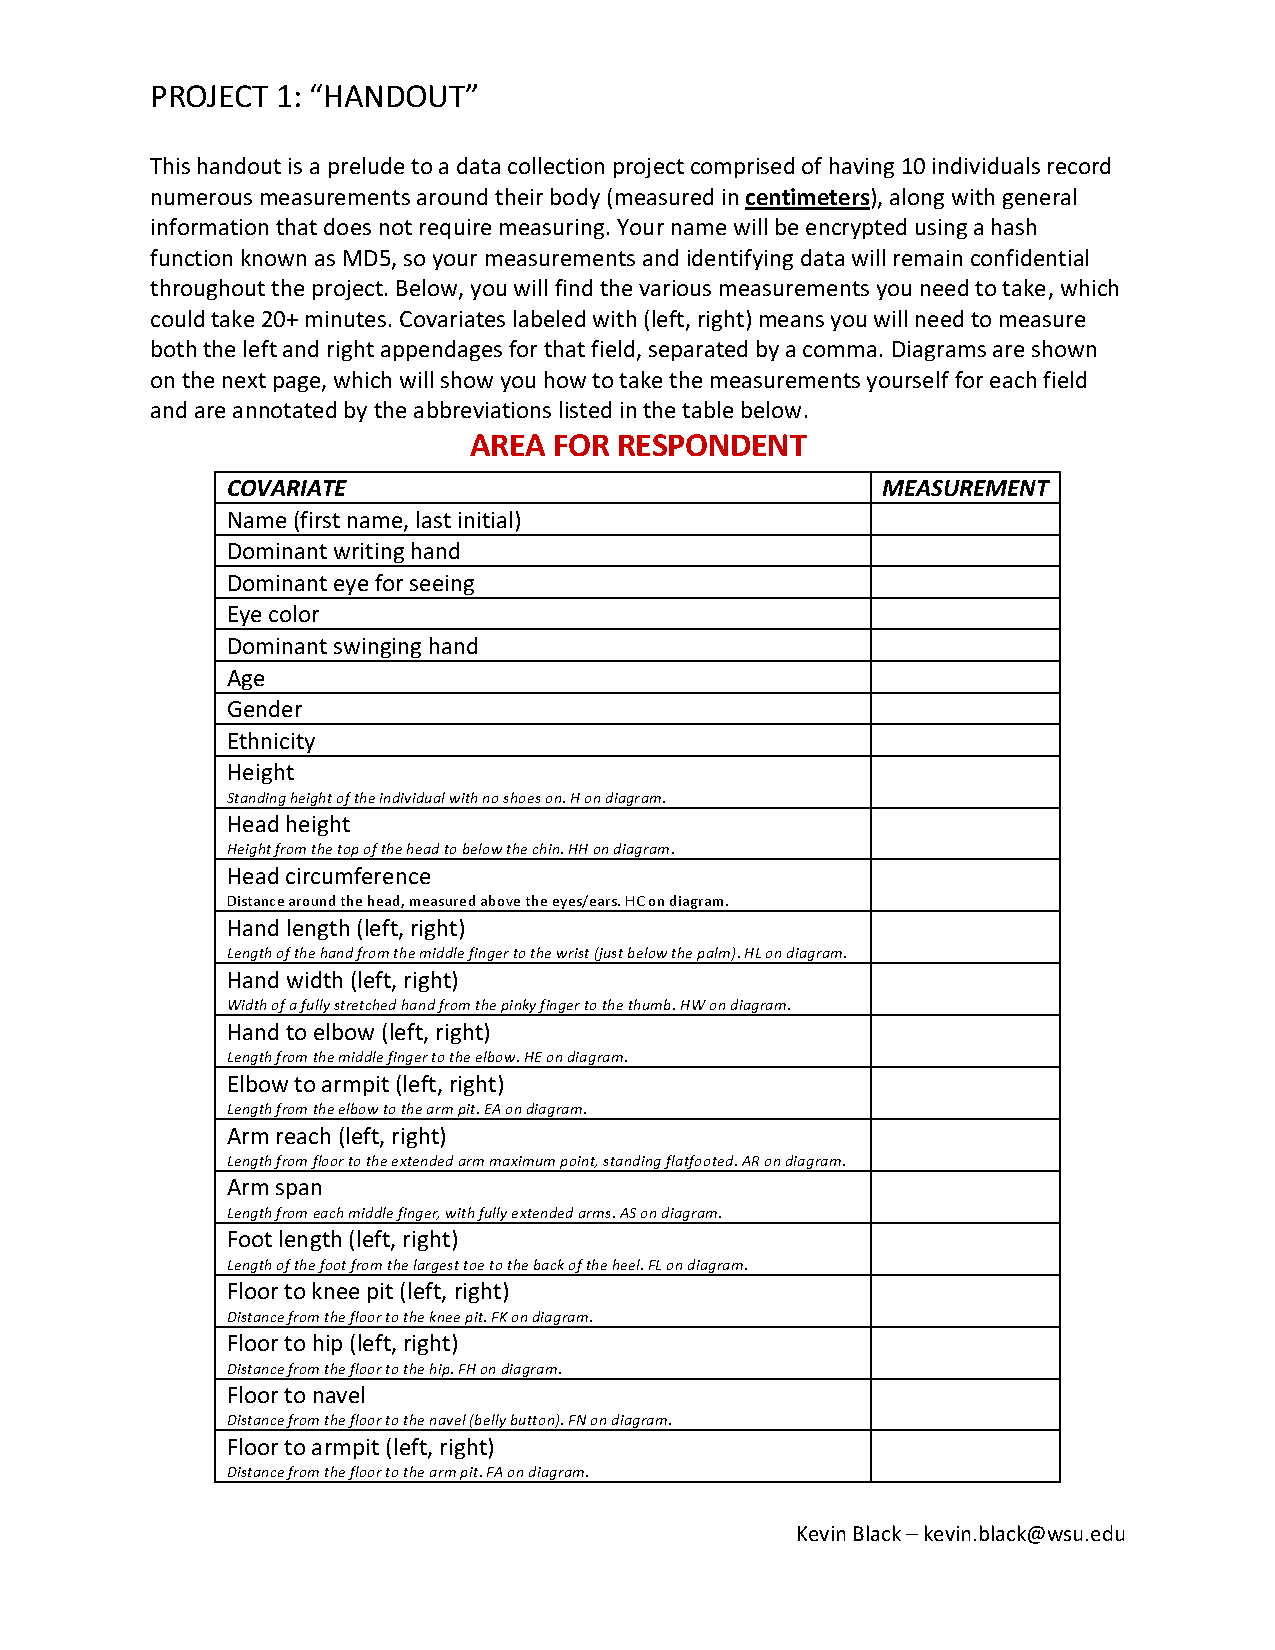
\includegraphics[trim = 0 0 0 0,clip,width=0.85\textwidth]{pdfs/handout1.pdf} }
    \end{center}
    \label{fig:handout-1}
    \hrule
\end{figure}

\newpage

\begin{figure}[!ht]
    \hrule
    \caption{ \textbf{Handout Page 2} }
    \begin{center}
        \scalebox{1.00}{    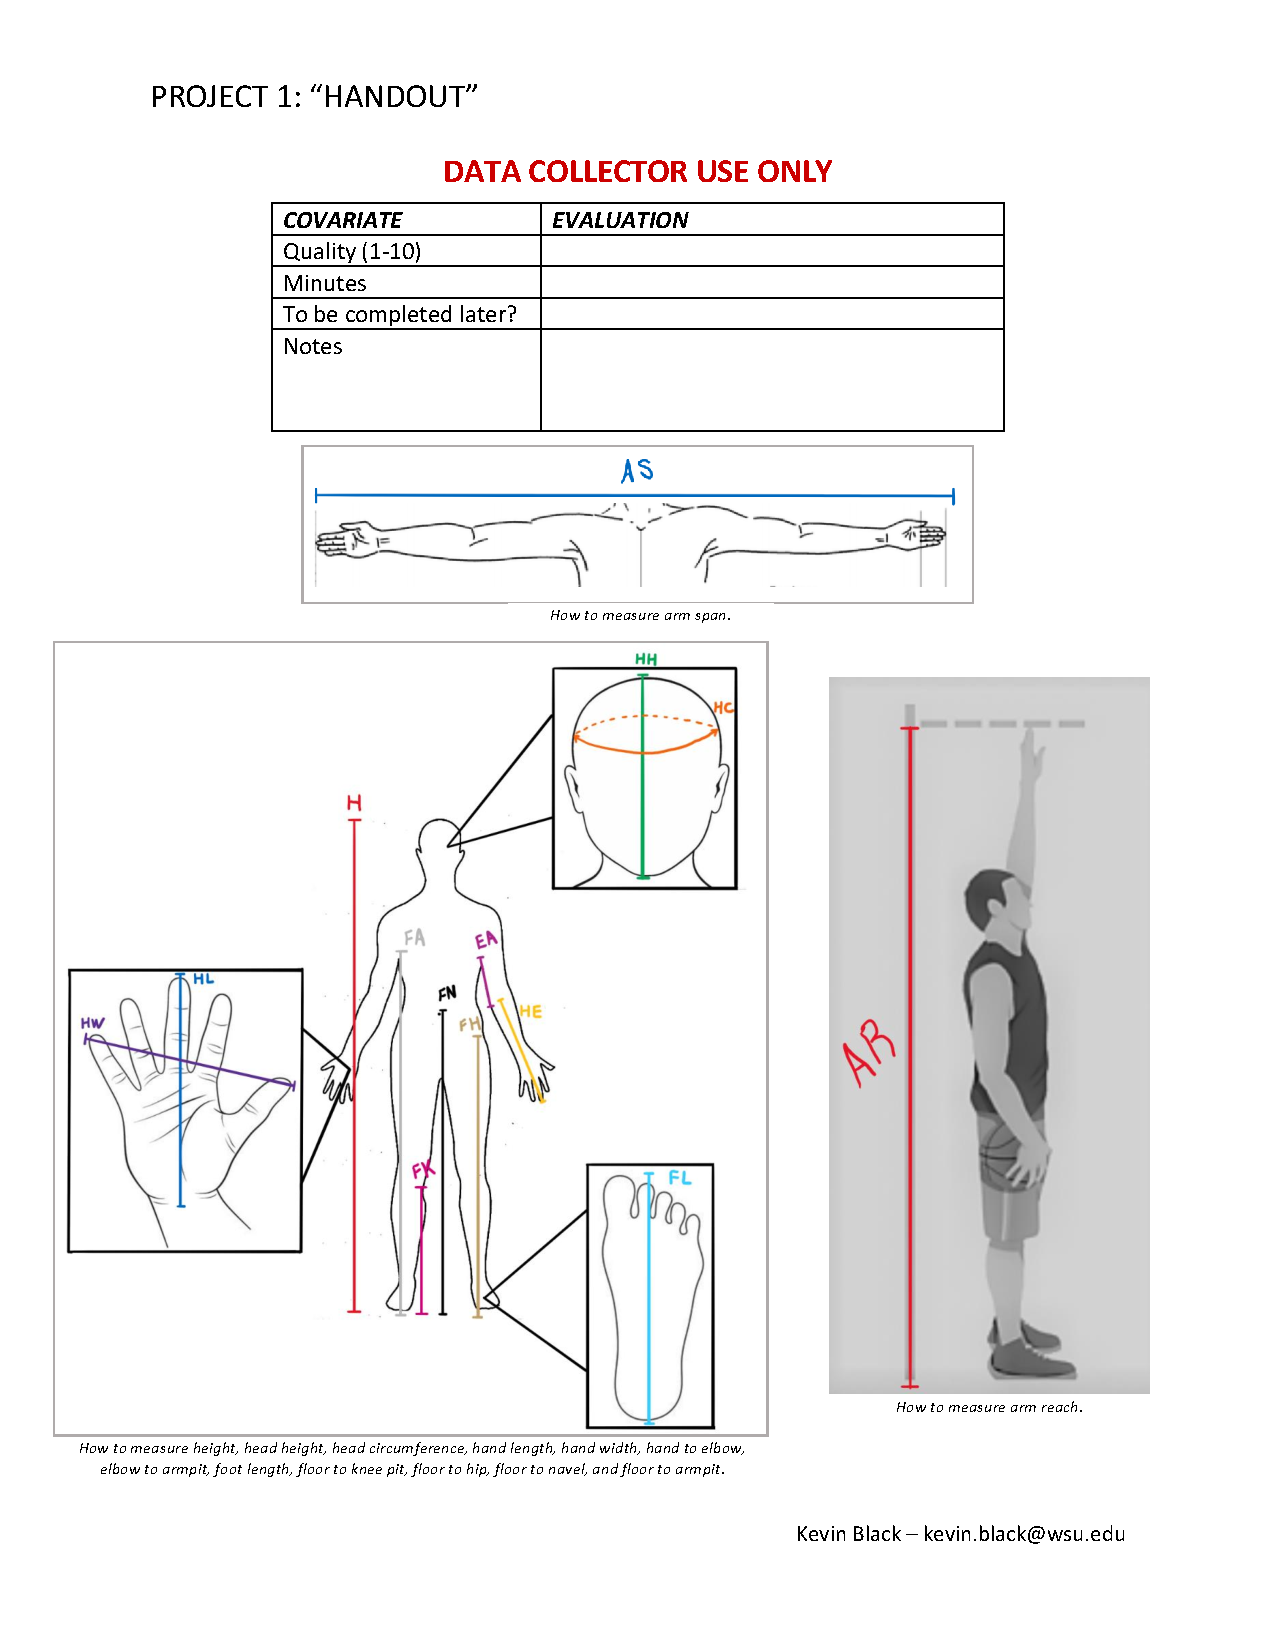
\includegraphics[trim = 0 0 0 0,clip,width=0.85\textwidth]{pdfs/handout2.pdf} }
    \end{center}
    \label{fig:handout-2}
    \hrule
\end{figure}

\newpage

\subsection{Data Set Explained}
\label{sec:appendix-dataset-ex}

In addition to how the data set was described in Section \ref{sec:data},
explanations regarding each attribute can be found below. After the
collaborative effort of all students having their data compiled, the
data set ended up having 428 total observations. However, the data set
was filled with an enormous amount of NA values in the body
measurements, potentially due to the time constraints of some students
or lack of attempt to fill out all fields. As a result, running the
function \texttt{complete.cases()} on the data set during the data
cleaning process returned a data frame containing only 262 observations,
about 61.21\% of the original data set size. \texttt{complete.cases()}
was used over \texttt{na.omit()} because the latter function would omit
all rows containing NA values based on all columns, including the rows
where the non-body measurement attributes had NA values, whereas the
former function would omit NA values only for the specified body
measurement columns.

\begin{figure}[!ht]
    \caption{ \textbf{Description of Each Field} }
    \begin{center}
        \scalebox{1.00}{    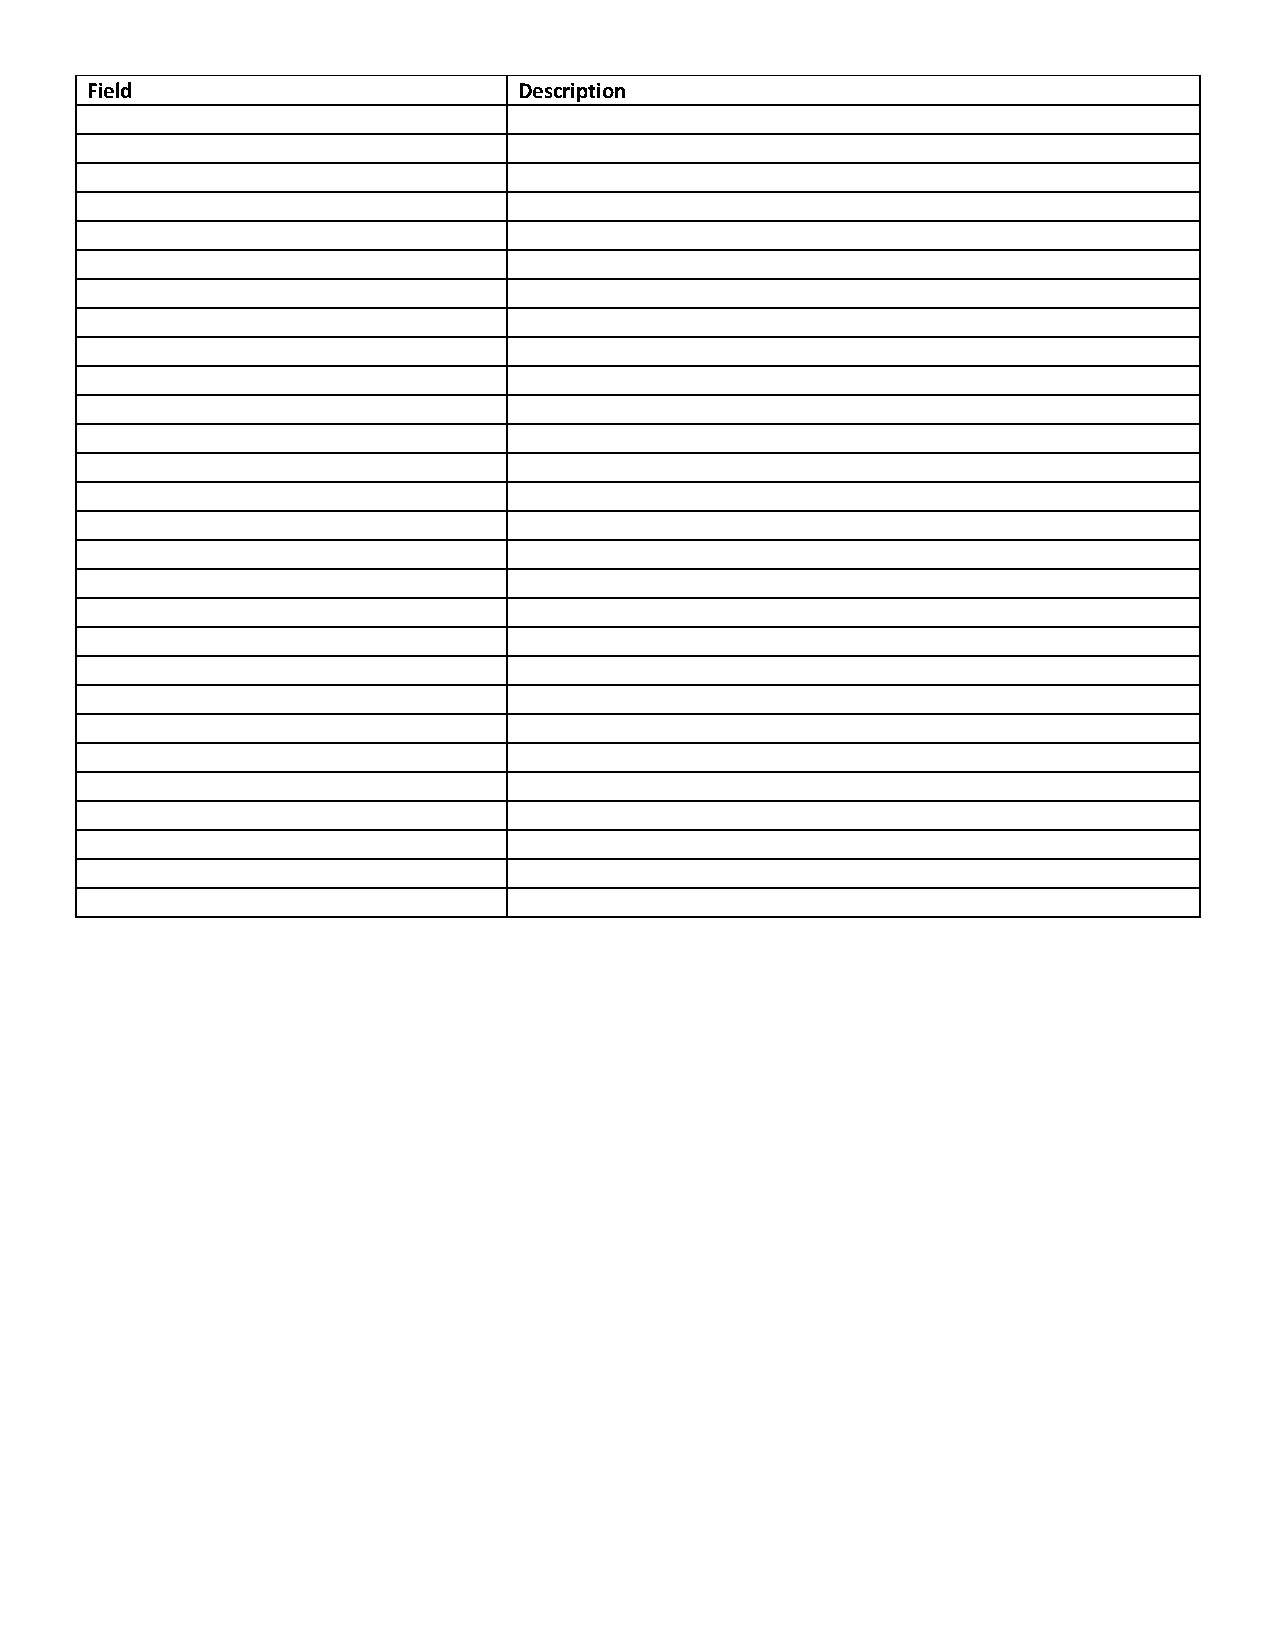
\includegraphics[trim = 0 350 100 35,clip,width=0.85\textwidth]{pdfs/datasets_explained.pdf} }
    \end{center}
    \label{fig:datasets_explained}
\end{figure}

\newpage

\subsection{R Code Used for Research}
\label{sec:r-setup}

\subsubsection{Sourced Functions}
\label{sec:functions}

\begin{Shaded}
\begin{Highlighting}[]
\NormalTok{prepareMeasureData =}\StringTok{ }\ControlFlowTok{function}\NormalTok{(measure,scale)\{}
  \CommentTok{\# Cleaning: omit NA rows based measured values, not on $side}
\NormalTok{  measure =}\StringTok{ }\NormalTok{measure[}\KeywordTok{complete.cases}\NormalTok{(measure[,}\DecValTok{4}\OperatorTok{:}\DecValTok{26}\NormalTok{]),]}
  
  \CommentTok{\# Cleaning: consistent naming convention}
\NormalTok{  measure}\OperatorTok{$}\NormalTok{gender =}\StringTok{ }\KeywordTok{factor}\NormalTok{(}\KeywordTok{tolower}\NormalTok{(measure}\OperatorTok{$}\NormalTok{gender))}
\NormalTok{  measure}\OperatorTok{$}\NormalTok{gender[measure}\OperatorTok{$}\NormalTok{gender}\OperatorTok{==}\StringTok{"f"}\NormalTok{] =}\StringTok{ "female"}
\NormalTok{  measure}\OperatorTok{$}\NormalTok{gender[measure}\OperatorTok{$}\NormalTok{gender}\OperatorTok{==}\StringTok{"m"}\NormalTok{] =}\StringTok{ "male"}
\NormalTok{  measure}\OperatorTok{$}\NormalTok{units =}\StringTok{ }\KeywordTok{factor}\NormalTok{(}\KeywordTok{tolower}\NormalTok{(measure}\OperatorTok{$}\NormalTok{units))}
\NormalTok{  measure}\OperatorTok{$}\NormalTok{units[measure}\OperatorTok{$}\NormalTok{units}\OperatorTok{==}\StringTok{"inches"}\NormalTok{] =}\StringTok{ "in"}
\NormalTok{  measure}\OperatorTok{$}\NormalTok{units[measure}\OperatorTok{$}\NormalTok{units}\OperatorTok{==}\StringTok{"inch"}\NormalTok{] =}\StringTok{ "in"}
\NormalTok{  measure}\OperatorTok{$}\NormalTok{units[measure}\OperatorTok{$}\NormalTok{units}\OperatorTok{==}\StringTok{"}\CharTok{\textbackslash{}"}\StringTok{in}\CharTok{\textbackslash{}"}\StringTok{"}\NormalTok{] =}\StringTok{ "in"}
\NormalTok{  measure}\OperatorTok{$}\NormalTok{units[measure}\OperatorTok{$}\NormalTok{units}\OperatorTok{==}\StringTok{"cm"}\NormalTok{] =}\StringTok{ "in"}
  
  \CommentTok{\# Converting cm to inches}
  \ControlFlowTok{for}\NormalTok{(row }\ControlFlowTok{in} \DecValTok{1}\OperatorTok{:}\KeywordTok{nrow}\NormalTok{(measure))\{}
    \ControlFlowTok{if}\NormalTok{(measure[row,]}\OperatorTok{$}\NormalTok{units}\OperatorTok{==}\StringTok{"cm"}\NormalTok{)\{}
\NormalTok{      measure[row,}\DecValTok{4}\OperatorTok{:}\DecValTok{26}\NormalTok{] \textless{}{-}}\StringTok{ }\NormalTok{measure[row,}\DecValTok{4}\OperatorTok{:}\DecValTok{26}\NormalTok{]}\OperatorTok{/}\FloatTok{2.54}
\NormalTok{    \}}
\NormalTok{  \}}
  
  \CommentTok{\# Scale data if scale = TRUE}
  \ControlFlowTok{if}\NormalTok{(scale)\{}
\NormalTok{    measure[,}\DecValTok{4}\OperatorTok{:}\DecValTok{26}\NormalTok{] \textless{}{-}}\StringTok{ }\KeywordTok{scale}\NormalTok{(measure[,}\DecValTok{4}\OperatorTok{:}\DecValTok{26}\NormalTok{])}
    \KeywordTok{return}\NormalTok{(measure)}
\NormalTok{  \} }\ControlFlowTok{else}\NormalTok{\{ }\CommentTok{\# If false, return without scaling}
    \KeywordTok{return}\NormalTok{(measure)}
\NormalTok{  \}}
\NormalTok{\}}

\NormalTok{read.file =}\StringTok{ }\ControlFlowTok{function}\NormalTok{(path,scale)\{}
  \KeywordTok{tryCatch}\NormalTok{(}
    \DataTypeTok{expr =}\NormalTok{ \{}
      \CommentTok{\# Open cleaned file if already available}
\NormalTok{      measure =}\StringTok{ }\NormalTok{utils}\OperatorTok{::}\KeywordTok{read.csv}\NormalTok{(}\KeywordTok{paste0}\NormalTok{(path.to.secret,}\StringTok{"measure{-}clean.txt"}\NormalTok{),}
                                \DataTypeTok{header =} \OtherTok{TRUE}\NormalTok{, }\DataTypeTok{quote =} \StringTok{""}\NormalTok{, }\DataTypeTok{sep =} \StringTok{"|"}\NormalTok{)}
      \KeywordTok{return}\NormalTok{(measure)}
\NormalTok{    \},}
    \DataTypeTok{warning =} \ControlFlowTok{function}\NormalTok{(w)\{}
      \CommentTok{\# If no clean file, open original file}
\NormalTok{      measure =}\StringTok{ }\NormalTok{utils}\OperatorTok{::}\KeywordTok{read.csv}\NormalTok{(}\KeywordTok{paste0}\NormalTok{(path.to.secret,}\StringTok{"measure{-}students.txt"}\NormalTok{),}
                                \DataTypeTok{header =} \OtherTok{TRUE}\NormalTok{, }\DataTypeTok{quote =} \StringTok{""}\NormalTok{, }\DataTypeTok{sep =} \StringTok{"|"}\NormalTok{)}
      \CommentTok{\# Clean data}
\NormalTok{      measure =}\StringTok{ }\KeywordTok{prepareMeasureData}\NormalTok{(measure,scale)}
      
      \CommentTok{\# Save cleaned data for later}
      \KeywordTok{write.table}\NormalTok{(measure,}\KeywordTok{paste0}\NormalTok{(path.to.secret,}\StringTok{"measure{-}clean.txt"}\NormalTok{),}\DataTypeTok{sep=}\StringTok{"|"}\NormalTok{,}\DataTypeTok{quote=}\OtherTok{FALSE}\NormalTok{)}
      \KeywordTok{return}\NormalTok{(measure)}
\NormalTok{    \}}
\NormalTok{  )    }
\NormalTok{\}}
\end{Highlighting}
\end{Shaded}

\subsubsection{Libraries, Sourcing Functions, Isolating Sexes}
\label{sec:sourcing}

\begin{Shaded}
\begin{Highlighting}[]
\CommentTok{\# Import necessary libraries}
\KeywordTok{library}\NormalTok{(stats) }\CommentTok{\# For cor()}
\KeywordTok{library}\NormalTok{(devtools) }\CommentTok{\# For source\_url()}
\KeywordTok{library}\NormalTok{(humanVerseWSU)}
\KeywordTok{library}\NormalTok{(Hmisc)}

\CommentTok{\# Source cleaning function}
\NormalTok{path.hub =}\StringTok{ "https://raw.githubusercontent.com/KevnBlack/WSU\_STATS419\_FALL2020/"}
\KeywordTok{source\_url}\NormalTok{(}\KeywordTok{paste0}\NormalTok{(path.hub,}\StringTok{"master/functions/functions{-}project{-}measure.R"}\NormalTok{))}

\CommentTok{\# Source Monte Shaffer function which builds correlation table}
\NormalTok{path.humanVerseWSU =}\StringTok{ "https://raw.githubusercontent.com/MonteShaffer/humanVerseWSU/"}
\KeywordTok{source\_url}\NormalTok{(}\KeywordTok{paste0}\NormalTok{(path.humanVerseWSU,}\StringTok{"master/misc/functions{-}project{-}measure.R"}\NormalTok{))}
\NormalTok{path.to.secret =}\StringTok{ "D:/School/Fall 2020/STAT 419/datasets/"}

\CommentTok{\# If changing scale value, be sure to remove previous measure file from working directory}
\NormalTok{measure.df =}\StringTok{ }\KeywordTok{read.file}\NormalTok{(path.to.secret,}\OtherTok{FALSE}\NormalTok{) }\CommentTok{\# Import data without scaling}
\KeywordTok{set.seed}\NormalTok{(}\DecValTok{1}\NormalTok{) }\CommentTok{\# Sample 200 observations from data frame}
\NormalTok{measure.sample =}\StringTok{ }\NormalTok{measure.df[}\KeywordTok{sample}\NormalTok{(}\KeywordTok{nrow}\NormalTok{(measure.df),}\DecValTok{200}\NormalTok{),]}

\CommentTok{\# Isolate male and female data}
\NormalTok{measure.df.m =}\StringTok{ }\NormalTok{measure.sample[measure.sample}\OperatorTok{$}\NormalTok{gender }\OperatorTok{==}\StringTok{ "male"}\NormalTok{,]}
\NormalTok{measure.df.f =}\StringTok{ }\NormalTok{measure.sample[measure.sample}\OperatorTok{$}\NormalTok{gender }\OperatorTok{==}\StringTok{ "female"}\NormalTok{,]}
\end{Highlighting}
\end{Shaded}

\subsubsection{First Research Subquestion}
\label{sec:first-subq}

\begin{Shaded}
\begin{Highlighting}[]
\CommentTok{\# Checking for normality}
\KeywordTok{shapiro.test}\NormalTok{(measure.df.m}\OperatorTok{$}\NormalTok{height.NA)}
\KeywordTok{shapiro.test}\NormalTok{(measure.df.m}\OperatorTok{$}\NormalTok{arm.span.NA)}
\KeywordTok{shapiro.test}\NormalTok{(measure.df.f}\OperatorTok{$}\NormalTok{height.NA)}
\KeywordTok{shapiro.test}\NormalTok{(measure.df.f}\OperatorTok{$}\NormalTok{arm.span.NA)}

\CommentTok{\# Correlation values between height and arm span}
\NormalTok{cor.m.has =}\StringTok{ }\KeywordTok{cor.test}\NormalTok{(measure.df.m}\OperatorTok{$}\NormalTok{height.NA, measure.df.m}\OperatorTok{$}\NormalTok{arm.span.NA)}
\NormalTok{cor.f.has =}\StringTok{ }\KeywordTok{cor.test}\NormalTok{(measure.df.f}\OperatorTok{$}\NormalTok{height.NA, measure.df.f}\OperatorTok{$}\NormalTok{arm.span.NA)}

\CommentTok{\# Graphs with correlation values and trend lines, for males and females}
\KeywordTok{par}\NormalTok{(}\DataTypeTok{mfrow =} \KeywordTok{c}\NormalTok{(}\DecValTok{1}\NormalTok{,}\DecValTok{2}\NormalTok{))}
\KeywordTok{plot}\NormalTok{(measure.df.m}\OperatorTok{$}\NormalTok{height.NA, measure.df.m}\OperatorTok{$}\NormalTok{arm.span.NA,}
     \DataTypeTok{main =} \KeywordTok{paste}\NormalTok{(}\StringTok{"Correlation ="}\NormalTok{, }\KeywordTok{round}\NormalTok{(cor.m.has}\OperatorTok{$}\NormalTok{estimate,}\DecValTok{5}\NormalTok{)), }\DataTypeTok{pch =} \DecValTok{4}\NormalTok{,}
     \DataTypeTok{xlab =} \StringTok{"Male Height (in)"}\NormalTok{, }\DataTypeTok{ylab =} \StringTok{"Male Arm Span (in)"}\NormalTok{, }\DataTypeTok{col =} \StringTok{"blue"}\NormalTok{)}
\KeywordTok{abline}\NormalTok{(}\KeywordTok{lm}\NormalTok{(measure.df.m}\OperatorTok{$}\NormalTok{height.NA }\OperatorTok{\textasciitilde{}}\StringTok{ }\NormalTok{measure.df.m}\OperatorTok{$}\NormalTok{arm.span.NA))}

\KeywordTok{plot}\NormalTok{(measure.df.f}\OperatorTok{$}\NormalTok{height.NA, measure.df.f}\OperatorTok{$}\NormalTok{arm.span.NA,}
     \DataTypeTok{main =} \KeywordTok{paste}\NormalTok{(}\StringTok{"Correlation ="}\NormalTok{, }\KeywordTok{round}\NormalTok{(cor.f.has}\OperatorTok{$}\NormalTok{estimate,}\DecValTok{5}\NormalTok{)), }\DataTypeTok{pch =} \DecValTok{0}\NormalTok{,}
     \DataTypeTok{xlab =} \StringTok{"Female Height (in)"}\NormalTok{, }\DataTypeTok{ylab =} \StringTok{"Female Arm Span (in)"}\NormalTok{, }\DataTypeTok{col =} \StringTok{"red"}\NormalTok{)}
\KeywordTok{abline}\NormalTok{(}\KeywordTok{lm}\NormalTok{(measure.df.f}\OperatorTok{$}\NormalTok{height.NA }\OperatorTok{\textasciitilde{}}\StringTok{ }\NormalTok{measure.df.f}\OperatorTok{$}\NormalTok{arm.span.NA))}
\end{Highlighting}
\end{Shaded}

\subsubsection{Second Research Subquestion}
\label{sec:second-subq}

\begin{Shaded}
\begin{Highlighting}[]
\CommentTok{\# Checking for normality}
\KeywordTok{shapiro.test}\NormalTok{(measure.df.m}\OperatorTok{$}\NormalTok{head.height.NA) }
\KeywordTok{shapiro.test}\NormalTok{(measure.df.m}\OperatorTok{$}\NormalTok{height.NA)}
\KeywordTok{shapiro.test}\NormalTok{(measure.df.f}\OperatorTok{$}\NormalTok{head.height.NA)}
\KeywordTok{shapiro.test}\NormalTok{(measure.df.f}\OperatorTok{$}\NormalTok{height.NA)}

\CommentTok{\# T.test to compare means of populations}
\KeywordTok{t.test}\NormalTok{(measure.df.m}\OperatorTok{$}\NormalTok{head.height.NA, measure.df.f}\OperatorTok{$}\NormalTok{head.height.NA)}
\KeywordTok{t.test}\NormalTok{(measure.df.m}\OperatorTok{$}\NormalTok{height.NA, measure.df.f}\OperatorTok{$}\NormalTok{height.NA)}

\CommentTok{\#\# How many \textquotesingle{}heads\textquotesingle{} on average is a male relative to their \textquotesingle{}height\textquotesingle{}?}
\KeywordTok{mean}\NormalTok{(measure.df.m}\OperatorTok{$}\NormalTok{height.NA)}\OperatorTok{/}\KeywordTok{mean}\NormalTok{(measure.df.m}\OperatorTok{$}\NormalTok{head.height.NA)}
\CommentTok{\#\# How many \textquotesingle{}heads\textquotesingle{} on average is a female relative to their \textquotesingle{}height\textquotesingle{}?}
\KeywordTok{mean}\NormalTok{(measure.df.f}\OperatorTok{$}\NormalTok{height.NA)}\OperatorTok{/}\KeywordTok{mean}\NormalTok{(measure.df.f}\OperatorTok{$}\NormalTok{head.height.NA)}
\end{Highlighting}
\end{Shaded}

\subsubsection{Correlation Table Creation}
\label{sec:males-corr}

\begin{Shaded}
\begin{Highlighting}[]
\CommentTok{\# Set up paths for tables}
\NormalTok{path.project =}\StringTok{ "D:/School/Fall 2020/STAT 419/git/WSU\_STATS419\_FALL2020/PROJECT{-}01/"}
\NormalTok{path.tables =}\StringTok{ }\KeywordTok{paste0}\NormalTok{(path.project,}\StringTok{"tables/"}\NormalTok{)}
  \KeywordTok{createDirRecursive}\NormalTok{(path.tables)}

\NormalTok{file.correlation =}\StringTok{ }\KeywordTok{paste0}\NormalTok{(path.tables,}\StringTok{"measure{-}table{-}m.tex"}\NormalTok{) }
\NormalTok{myData =}\StringTok{ }\KeywordTok{as.matrix}\NormalTok{(measure.df.m[,}\KeywordTok{c}\NormalTok{(}\StringTok{"height.NA"}\NormalTok{,}\StringTok{"head.height.NA"}\NormalTok{,}\StringTok{"arm.span.NA"}\NormalTok{)])}

\CommentTok{\# Create male table}
\KeywordTok{buildLatexCorrelationTable}\NormalTok{(myData, }
  \DataTypeTok{rotateTable =} \OtherTok{FALSE}\NormalTok{,}
  \DataTypeTok{width.table =} \FloatTok{0.95}\NormalTok{, }\CommentTok{\# 0.95 when rotateTable is FALSE, 0.60 when TRUE}
  \DataTypeTok{myFile =}\NormalTok{ file.correlation,}
  \DataTypeTok{myNames =} \KeywordTok{c}\NormalTok{(}\StringTok{"Height (in)"}\NormalTok{, }\StringTok{"Head Height (in)"}\NormalTok{, }\StringTok{"Arm Span (in)"}\NormalTok{),}
  \DataTypeTok{myCaption =} \StringTok{"Descriptive Statistics and Correlation Analysis for Males"}\NormalTok{)}

\KeywordTok{Sys.sleep}\NormalTok{(}\DecValTok{2}\NormalTok{) }\CommentTok{\# Error checking when knitting{-}to{-}pdf}

\NormalTok{file.correlation =}\StringTok{ }\KeywordTok{paste0}\NormalTok{(path.tables,}\StringTok{"measure{-}table{-}f.tex"}\NormalTok{)}
\NormalTok{myData =}\StringTok{ }\KeywordTok{as.matrix}\NormalTok{(measure.df.f[,}\KeywordTok{c}\NormalTok{(}\StringTok{"height.NA"}\NormalTok{,}\StringTok{"head.height.NA"}\NormalTok{,}\StringTok{"arm.span.NA"}\NormalTok{)])}

\CommentTok{\# Repeat for females}
\KeywordTok{buildLatexCorrelationTable}\NormalTok{(myData, }
  \DataTypeTok{rotateTable =} \OtherTok{FALSE}\NormalTok{,}
  \DataTypeTok{width.table =} \FloatTok{0.95}\NormalTok{,}
  \DataTypeTok{myFile =}\NormalTok{ file.correlation,}
  \DataTypeTok{myNames =} \KeywordTok{c}\NormalTok{(}\StringTok{"Height (in)"}\NormalTok{, }\StringTok{"Head Height (in)"}\NormalTok{, }\StringTok{"Arm Span (in)"}\NormalTok{),}
  \DataTypeTok{myCaption =} \StringTok{"Descriptive Statistics and Correlation Analysis for Females"}\NormalTok{)}

\KeywordTok{Sys.sleep}\NormalTok{(}\DecValTok{2}\NormalTok{)}
\end{Highlighting}
\end{Shaded}

\newpage

\subsubsection{Tables of Descriptive Statistics and Correlations}
\label{sec:correlation-tables}
\begin{table}[!htbp]
\footnotesize
\centering
\caption{\textbf{Descriptive Statistics and Correlation Analysis for Males}}
\label{table:correlation}
\begin{tabularx}{0.95\textwidth}{{r@{ \ \ } p{35mm} r@{}lp{1mm} r@{}l p{5mm} r@{}l p{2mm} r@{}l p{2mm}   r@{}l  }}
 & \\
\hline
 & \\
\multicolumn{2}{c}{\textbf{ }} & \multicolumn{2}{c}{\textbf{M}} & & \multicolumn{2}{c}{\textbf{SD}} &  & \multicolumn{2}{c}{\textbf{1}} &  & \multicolumn{2}{c}{\textbf{2}} &  & \\ 
 & \\
\hline
 & \\
\textbf{1} & \textbf{Height (in)} &  138&.7 &  &  53&.34 &  &  1&  &  &  \multicolumn{2}{c}{ \  \  \  \  \ }  &  & \\ 
 & \\
\textbf{2} & \textbf{Head Height (in)} &  18&.2 &  &  7&.06 &  &  &.97{$^{***}$}  &  &  1&  &  & \\ 
 & \\
\textbf{3} & \textbf{Arm Span (in)} &  140&.1 &  &  55&.67 &  &  &.96{$^{***}$}  &  &  &.90{$^{***}$}  &  & \\ 
 & \\
\hline
 & \\
\multicolumn{13}{p{0.86\textwidth}}{  \footnotesize { \begin{hangparas}{0.75in}{1} \textbf{\underline{Notes}:} \ \ Pearson pairwise correlations are reported; \newline a two-side test was performed to report correlation significance.  \end{hangparas} } }  & \\  
\multicolumn{13}{p{0.86\textwidth}}{  {\tiny {$^{\dagger} p < .10$} }  {     } {\tiny        {$^{*} p < .05$} }  {     } {\tiny       {$^{**} p < .01$} }  {     } {\tiny      {$^{***} p < .001$} } {     }     } & \\ 
 & \\
\hline
\end{tabularx}
\end{table}

\begin{table}[!htbp]
\footnotesize
\centering
\caption{\textbf{Descriptive Statistics and Correlation Analysis for Females}}
\label{table:correlation}
\begin{tabularx}{0.95\textwidth}{{r@{ \ \ } p{35mm} r@{}lp{1mm} r@{}l p{5mm} r@{}l p{2mm} r@{}l p{2mm}   r@{}l  }}
 & \\
\hline
 & \\
\multicolumn{2}{c}{\textbf{ }} & \multicolumn{2}{c}{\textbf{M}} & & \multicolumn{2}{c}{\textbf{SD}} &  & \multicolumn{2}{c}{\textbf{1}} &  & \multicolumn{2}{c}{\textbf{2}} &  & \\ 
 & \\
\hline
 & \\
\textbf{1} & \textbf{Height (in)} &  107&.5 &  &  54&.08 &  &  1&  &  &  \multicolumn{2}{c}{ \  \  \  \  \ }  &  & \\ 
 & \\
\textbf{2} & \textbf{Head Height (in)} &  14&.3 &  &  6&.90 &  &  &.96{$^{***}$}  &  &  1&  &  & \\ 
 & \\
\textbf{3} & \textbf{Arm Span (in)} &  105&.2 &  &  55&.84 &  &  &.97{$^{***}$}  &  &  &.94{$^{***}$}  &  & \\ 
 & \\
\hline
 & \\
\multicolumn{13}{p{0.86\textwidth}}{  \footnotesize { \begin{hangparas}{0.75in}{1} \textbf{\underline{Notes}:} \ \ Pearson pairwise correlations are reported; \newline a two-side test was performed to report correlation significance.  \end{hangparas} } }  & \\  
\multicolumn{13}{p{0.86\textwidth}}{  {\tiny {$^{\dagger} p < .10$} }  {     } {\tiny        {$^{*} p < .05$} }  {     } {\tiny       {$^{**} p < .01$} }  {     } {\tiny      {$^{***} p < .001$} } {     }     } & \\ 
 & \\
\hline
\end{tabularx}
\end{table}


\newpage




%% appendices go here!


\newpage
\theendnotes

%%%%%%%%%%%%%%%%%%%%%%%%%%%%%%%%%%%  biblio %%%%%%%%
\newpage
\begin{auxmulticols}{2}
\singlespacing 
\bibliography{./../biblio/master.bib}

%%%%%%%%%%%%%%%%%%%%%%%%%%%%%%%%%%%  biblio %%%%%%%%
\end{auxmulticols}

\newpage
{
\hypersetup{linkcolor=black}
\setcounter{tocdepth}{3}
\tableofcontents
}



\end{document}